% !TEX program = xelatex
\chapter{Grundlagen}
\label{ch:basics}

\section{Lokalisierungsverfahren}

Lokalisieren bedeutet immer, eine Pose innerhalb einer Umgebung zu bestimmen. Bei einigen Verfahren ist die Umgebung bekannt weil eine Karte gegeben ist, bei anderen ist die Umgebung unbekannt.
\newline

Prinzipiell werden Lokalisierungsverfahren anhand der Aufgabenstellung in zwei Kategorien unterschieden. Zum einen gibt es globale Verfahren und zum anderen Position Tracking bzw lokale Verfahren. Die Assoziation global und lokal bezieht sich auf das Koordinatensystem bzw Frame zu dem Bezug genommen wird.

\subsection{Globale Lokalisierung}

Globale Lokalisierung schätzt die Pose im globalen Referenzsystem, d.h. in Bezug zum Koordinatenursprung der Umgebungskarte. Dabei müssen die Wahrscheinlichkeiten für mögliche Posen geschätzt werden. Ein bekanntes Beispiel für globale Lokalisierungsverfahren ist die Markov Lokalisation.
\newline

Eine Aufgabe, in dem die globalen Lokalisierung angewendet wird, ist die Ermittelung der Startposition. Denn autonome Agenten müssen sich häufig orientieren, nachdem sie durch externe Kräfte bewegt wurden. Globale Lokalisierung löst beispielsweise das Kidnapped-Robot Problem, bei dem der Agent plötzlich versetzt wurde oder bestimmt den Zustand nach dem Anschalten. Der Wake-Up eines Roboters zählt als ein Sonderfall des Kidnapped-Roboters, wobei dem Agenten hier i.d.R. bekannt ist, dass sich seine Position verändert hat.
\newline

Globalen Lokalisierungsverfahren müssen also in der Lage sein auch gro{\ss}e Positionsänderungen kompensiert zu können. \cite{locFox}


\subsection{Position Tracking}
Beim Position Tracking ist die Ausgangsposition in der Regel ungefähr bekannt und es sollen vor allem odometrische Fehler korrigiert werden. Der Referenzrahmen des position Tracking ist lokal und muss in einem weiteren Schritt in das globalen (Welt) Koordinatensystem transformiert werden. 
\newline

Für das Position Tracking wird die Pose inkrementell, von Frame zu Frame, ermittelt. Daher führen zu gr{\ss}e Änderungen zwischen zwei Zuständen zum Ausfall und die Schätzung muss abgebrochen werden.
\newline

Visuelle Odometrie zählt zu den Position Tracking Verfahren. Die Startposition wird als Koordinatenursprung des lokalen Bezugssystems gesetzt. Die Odometrieschätzung der aktuellen Pose bezieht sich immer auf die vorherige Pose. 

%%%%%%%%%%%%%%%%%%%%%%%%%%%%%%%%%%%%%%%%%%%%%%%%%%%
\section{3-D Strukturen und Kamerapose aus 2-D Bildern}
In den vergangenen 30 Jahren wurde viel Forschung im Bereich der Computer Vision als ein Teilgebiet der autonomen Robotik betrieben. Werden die Umgebungsinformationen teilweise oder ausschlie{\ss}lich aus Kamerasensoren erhalten, können geometrische Modelle aufgestellt werden um Informationen aus den Bildern zu gewinnen. Grundsätzlich soll die Kamera Pose aus Pixelinformationen hergeleitet werden. Eine Grundlage hierfür bildet die Korrespondenzanalyse, für die Merkmale aus den Bildern extrahiert werden müssen. Durch Bildkorrespondenzen kann eine Beziehung zwischen Bildern und zwischen Kamera und Umwelt hergestellt werden. Beim Umgang mit Bildkorrespondenzen werden Methoden der Projektiven- und Epipolargeometrie herangezogen.
\begin{figure}[!ht]
  \centering
  \includegraphics[width=0.4\textwidth]{pictures/02_2dpane.png}
  \caption[Abbildung von 3-D zu 2-D]{Abbildung einer 3-D Punktes X auf den 2-D Punkt p der Bildebene. (Scaramuzza, 2011 \cite{ScFrVO})}
  \label{fig:2dpane}
\end{figure}

Transformationen aus der projektiven Geometrie können im Alltag regelmä{\ss}ig auf Fotos beobachtet werden.  Beispielsweise erscheint ein Kreis je nach Perspektive, aus der er Abgebildet wurde, in einem Bild als Ellipse. Der Kreis wurde transformiert.
\newline

Durch Kamerasensoren werden Objekte aus dem 3-Dimensionalen Raum, der 'Welt', auf die 2-Dimensionalen Bildebene des Kamerabildes abgebildet. Dabei bleiben fast keine Eigenschaften der transformierten Objekte erhalten. Wie beim bereits aufgeführten Beispiel Kreis als Ellipse werden Objekte deformiert. Die einzige Eigenschaft, die erhalten bleibt, ist die Geradentreue. D.h. gerade Linien bleiben auch im Projektiven Raum immer gerade Linien.
% 
%%%%%%%%%%%%%%%%%%%%%%%%%%%%%%%%%%%%%%%%%%%%%%%%%%%
\subsection{Koordinatensysteme}
Bekannt ist der Euklidische Raum und die Euklidische Geometrie als Beschreibung von Winkeln und Formen von Objekten. Meistens werden Punkte des euklidischen Raumes im kartesischen Koordinatensystem dargestellt. Ein Problem im Modell der euklidischer Geometrie sind parallele Linien. Als Sonderfall wird angenommen, das sich parallele Linien im Unendlichen schneiden. Obwohl es tatsächlich im Euklidischen Raum keine Punkte im Unendlichen gibt.
\newline 

Der Projektive Raum ist die Transformation des Euklidischen Raums durch Einführung der Punkte im Unendlichen. Die Punkte werden dort als ideale Punkte oder Fernpunkte bezeichnet. Auch Räume sind in der geometrischen Betrachtung Objekte, die rotiert, verschoben oder gestreckt werden können.
\newline
\begin{figure}[!ht]
  \begin{subfigure}[t]{0.45\textwidth}
    \centering
    \begin{equation}
      T_{rotation}(\theta) = 
      \begin{pmatrix}
        cos \theta & -sin \theta \\
        sin \theta & cos \theta 
      \end{pmatrix}
    \end{equation}
    \caption*{Transformation Rotation für 2-D}
    \end{subfigure}
  \hfill
  \begin{subfigure}[t]{0.45\textwidth}
    \centering
    \begin{equation}
      T_{scale}(S) = 
      \begin{pmatrix}
        Sx & 0 \\
        0 & Sy 
      \end{pmatrix}
    \end{equation}
    \caption*{Transformation Verschiebung für 2-D}
  \end{subfigure}
  \label{fig:lintrans}
\end{figure}

Transformationen sind Operationen die auf alle Objekte angewendet werden können, also auf den Raum ebenso wie auf den Punkt. Verschiebung und Rotation zählen zu den Lineartransformationen und lassen sich daher durch Matrizen beschreiben.

\subsubsection{Homogene Koordinaten}
Die Translation, eine wichtige Transformation die für Lokalisierung benötigt wird, ist nicht linear. Um Translation in Matritzenschreibweise darstellen zu können, muss von kartesischen Koordinaten $(x ,y)$ zu homogenen Koordinaten $(x, y, 1)$ übergegangen werden. Dabei wird ein Vektor um eine weitere Komponente $w = 1$ erweitert. Es handelt sich bei homogenen Koordinaten um eine andere Schreibweise, nicht um eine Veränderung der Dimension. Alle Punkte $(kx, ky, k)$ sind gleich, für $k \neq 0$. 

Eine Rücktransformation von homogenen Koordinaten zu kartesischen erfolgt durch division von $(x,y)$ durch $k$. 

% %
\begin{figure}[!ht]
  \centering
  \begin{subfigure}[t]{0.4\textwidth}
    \centering
    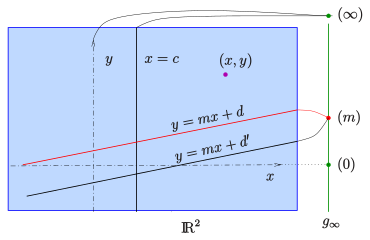
\includegraphics[width=\textwidth]{pictures/02_Projebeneinhomkoords.pdf}
    \caption[Projektive Ebene]{Die Projektive Ebene}
    \label{fig:y equals x}
  \end{subfigure}
  \hfill
  \begin{subfigure}[t]{0.55\textwidth}
    \centering
    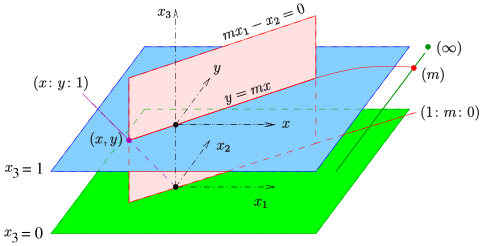
\includegraphics[width=\textwidth]{pictures/02_Projebenehomkoords.pdf}
    \caption[Urspungsgerade der inhomogenen Koordinaten]{Allen inhomogenen Geraden kann eine gemeinsame Ursprungsgerade $(1:m:0)$ zugeordnet werden}
    \label{fig:three sin x}
  \end{subfigure}
  \caption[Beziehung zwischen inhomogenen und homogenen Koordinaten]{Beziehung zwischen inhomogenen und homogenen Koordinaten, (Ag2gaeh Wikimedia Creative Commons)}
     \label{fig:three graphs}
\end{figure}

%
Es wurde bereits erwähnt, dass im projektiven Raum sog. Fernpunkte eingeführt werden um Unendlichkeit einzuführen. Im inhomogenen Modell treffen sich zwei parallele Geraden im Fernpunkt $\inf$ der als $m$ bezeichnet werden soll. $m$ ist Teil der Geradengleichung aller inhomogenen Geraden $y = mx + d$. 

In gleicher Weise kann $m$ auch allen Ursprungsgeraden aller Ursprungsebenen zugewiesen werden. Daraus folgt

\begin{equation}
  \begin{aligned}
    (x,y) &\rightarrow &(x:y:1) \\
    (m) &\rightarrow &(1:m:0)  \\
    (\inf) &\rightarrow &(0:1:0)
  \end{aligned}
\end{equation}

Durch dieses Schreibweise der Koordinaten wurde erreicht, dass es keine Ausnahmefälle mehr gibt. Bisherige Transformationen werden in homogenen Koordinaten geschrieben. Hiermit kann auch die Translation als lineare Abbildung beschrieben werden.

\begin{equ}[!ht]
  \begin{equation}
    \begin{pmatrix}
      x' \\ y' \\ w
      \end{pmatrix}
      = 
      \begin{pmatrix}
        Sx & 0 & 0\\
        0 & Sy & 0\\
        0 & 0 & 1
      \end{pmatrix}
      \begin{pmatrix}
        x \\ y \\ 1
      \end{pmatrix}
    \end{equation}
    \caption*{Verschiebung in Homogenen Koordinaten}
% \end{equ}

% \begin{equ}[!ht]
  \begin{equation}
    \begin{pmatrix}
      x' \\ y' \\ w
    \end{pmatrix}
    =
    \begin{pmatrix}
      xcos\theta & -ysin\theta & 0 \\
      xsin\theta & ycos\theta & 0 \\
      0 & 0 & 1
    \end{pmatrix}
     \begin{pmatrix}
      x \\ y \\ 1
    \end{pmatrix}
  \end{equation}
  \caption*{Rotation in Homogenen Koordinaten}
\end{equ}

\begin{equ}[!ht]
  \begin{equation}
    \begin{pmatrix}
      x' \\ y' \\ w
      \end{pmatrix}
      = 
      \begin{pmatrix}
        0 & 0 & a\\
        0 & 0 & b\\
        0 & 0 & 1
      \end{pmatrix}
      \begin{pmatrix}
        x \\ y \\ 1
      \end{pmatrix}
    \end{equation}
    \caption*{Translation in Homogenen Koordinaten}
  \end{equ}
\newpage

%%%%%%%%%%%%%%%%%%%%%%%%%%%%%%%%%%%%%%%%%%%%%%%%%%%%%%%%%%%%%%%%%%%%%%%%%%%%%%%
\subsubsection{Kameraprojektionen}
\begin{figure}
  \centering
    \includegraphics[width=0.45\textwidth]{pictures/02_projective_pane_model.png}
  \caption[Die Kameraprojektion]{Punkte und Linien in $\mathbb{P}^2$ aus $\mathbb{P}^3$ (Hartley, 2003 \cite{Hartley:MVG})}
\end{figure}
Das Abbilden von 3-D auf 2-D ist eine Projektion die durch eine Zentralprojektion beschrieben wird. Die Strahlen von allen Punkten laufen durch das Projektionszentrum, in diesem Fall der Brennpunkt. Der Brennpunkt ist gleichzeitig das Kamerazentrum. Dabei schneiden die Strahlen die Bildebene, die vor der Kamera aufgespannt wird. Die Schnittpunkte sind die Bildpunkte. Dieses Modell entspricht dem Modell der Lochbildkamera. D.h. Fokus und Linsenstärke werden vernachlässigt. 

In der projektiven Geometrie ist die Zentralprojektion eine Abbildung von $\mathbb{P}^3$ zu $\mathbb{P}^2$. Ein Punkt in  $\mathbb{P}^3$ kann als $(X, Y, Z, T)^T$ in homogenen Koordinaten geschrieben werden und das Projektionszentrum als $(0, 0, 0, 1)^T$. Um $\mathbb{P}^3$ auf $\mathbb{P}^2$ ab zu bilden kann die sogenannte Kameramatrix (oder Projektionsmatrix) P verwendet werden.\cite{Hartley:MVG} Es ergibt sich eine lineare Abbildung zwischen Kameraprojektion und einem Punkt im Raum als 

\begin{equation}
  \begin{pmatrix}
    x\\ y \\ w
  \end{pmatrix}
  = P_{3\times4}
  \begin{pmatrix}
    X\\Y\\Z\\T
  \end{pmatrix}
\end{equation}



%%%%%%%%%%%%%%%%%%%%%%%%%%%%%%%%%%%%%%%%%%%%%%%%%%%%%%%%%%%%%%%%%%%%%%%%%%%%%%%
\subsection{Korrespondenzanalyse}
Bildkorrespondenzen sind Merkmale in Bildern die das selbe Objekt in zwei unterschiedlichen Bildern beschreiben und als Ankerpunkte zwischen den Kamerapositionen dienen. Wenn eine Rekonstruktion von 3-D Punkten durchgeführt werden soll muss immer die Aufgabe der Bestimmung von Korrespondenzen gelöst werden.


Bei der Korrespondenzanalyse geht es ganz allgemein darum übereinstimmende Bildmerkmale in zwei Bildern zu finden. Handelt es sich um zwei Bilder einer Stereokamera, spezifiziert sich die Aufgabenstellung zur Stereoanalyse.

Die Korrespondenzanalyse ist aus dem Anwendungsgebiet der Bewegungsschätzung für Videostreaming hervorgegangen. Korrespondenzanalyse wird in der Videokodierung genutzt um zu Schätzen, in welchen Bereichen eines Bildes Bewegung stattgefunden hat. Für die Bereiche werden Bewegungsvektoren erstellt. Bilder werden anschlie{\ss}end mit den Bewegungsvektoren kodiert und so müssen nur Teile des Bildes übertragen und aktualisiert werden. \cite{stereoSchreer}  

Bei SfM und Visueller Odometrie soll im Grunde genau das Gegenteil erreicht werden. Die Szene ist überwiegend statisch und die Bewegung der Kamera muss geschätzt werden. Schwierigkeiten, die bei der Korrespondenzanalyse auftreten, sind beispielsweise Regionen die nur im Bildfeld einer Kamera vorhanden sind, aufgrund von Geometrie oder Verdeckung, wiederkehrende Muster oder Oberflächen mit schwacher Textur.
\newline

Die Korrespondenzanalyse kann in pixelbasierte und merkmalsbasierte Verfahren unterschieden werden. Für das erstellen der Disparitätenkarte (ein Schritt zur Ermittlung der Tiefenwerte von Pixeln) wird eine pixelbasierte Stereoanalyse verwendet. Zum einen, da eine hohe Informationsdichte benötigt wird. Zum anderen kann aus der Kenntnisse über die Geometrie des Stereoaufbaus die Suche auf einen eindimensionalen Suchraum beschränkt werden. Diese Aussage wird in der folgenden Betrachtung der Epipolargeometrie noch ersichtlich.
\newline

Für die Korrespondenzanalyse der Bewegungsschätzung werden merkmalsbasierte Verfahren angewendet.

%%%%%%%%%%%%%%%%%%%%%%%%%%%%%%%%%%%%%%%%%%%%%%%%%%%%%%%
\subsection{Verbinden von zwei Ansichten durch Epipolargeometrie}
\begin{center}
    \begin{figure}[!h]
      \centering
      \includegraphics[width=\textwidth]{pictures/epipane_01.png}
      \caption[Bildebenen mit Epipolarlinien]{(a) Die Kameras sind gekennzeichnet als $C$ und $C'$, vor Ihnen spannen sich die jeweiligen Bildebenen auf. 
      (b) X muss auf seiner Epipolarlinie liegen. (Hartley, 2003 \cite{Hartley:MVG})}
      \label{fig:epigem1}
    \end{figure}
\end{center}

Die Epipolargeometrie besagt, dass die Kamerazentren $C$ und $C'$, die Bildpunkte $x$ und $x'$ und die Raumpunkte koplanar sein müssen.
%
\begin{equation}
  Cx\cdot(C C' \times C x') = 0
  \label{eq:epi_const}
\end{equation}

Diese Forderung wird durch die Fundamentalmatrix $F$ abgebildet. Die Fundamentalmatrix wird als algebraische Repräsentation der Epipolargeometrie bezeichnet. Sie ist eine homogene $3 \times 3$ Matrix mit Rang(2), die nachfolgende Gleichung erfüllt \cite{Hartley:MVG} 

\begin{equation}
  {x'}^{T}Fx = 0
  \label{eq:fun}
\end{equation}

%
In Matrixschreibweise mit Homogenen Koordinaten lässt sich \ref{eq:fun} schreiben als

\begin{equation}
  \begin{bmatrix}
    {x_R}_i & {y_R}_i & 1
  \end{bmatrix}
  \begin{bmatrix}
    f_{11} & f_{12} & f_{13} \\
    f_{21} & f_{22} & f_{23} \\
    f_{31} & f_{32} & f_{33} \\
  \end{bmatrix}
  \begin{bmatrix}
    x_i \\
    y_i \\
    1
  \end{bmatrix}
  = 0
\end{equation}

Zwischen diesen koplanaren Punkten lässt sich eine Ebene aufspannen. Diese Ebene wird als Epipolarebene bezeichnet. Jede Kamera spannt au{\ss}erdem eine Bildebene in Blickrichtung auf. Die Epipolarebene schneidet die Bildebenen. Aus Sicht der ersten Kameraposition befindet sich $X$ auf einem Strahl der vom Projektionszentrum durch den Bildpunkt $x$ der Bildebene läuft. Dieser Strahl entspricht der Epipolarlinie im zweiten Bild, die durch die Epipolarebene geschnitten wird.
%%
%
Um einen Punkt eindeutig bestimmen zu können, lässt sich folgende Beschränkung einführen: $x'$ muss auf seiner Epipolarlinie $l'$ liegen um eine Projektion des Gleichen Punktes $X$ zu sein wie $x$.
\begin{equation}
  x \mapsto l' 
\end{equation}
Die Epipolarlinie ist die Überschneidung zwischen Epipolar- und Bildebene. Der Epipol ist der Punkt in der Bildebene in welchem diese die Basislinie schneidet. Die Baseline ist die Gerade die zwischen den Kamerazentren $C$ und $C'$ gezogen werden kann. 

%%%%%%%%%%%%%%%%%%%%%%%%%%%%%%%%%%%%%%%%%%%%%%%%
\subsection{Sonderfall Stereo Vision}
\begin{center}
    \begin{figure}[h!]
    	\centering
    	\includegraphics[width=.75\textwidth]{02_stereo.png}
    	\caption[Parallele Epipolarlinien]{Sind die Kamerazentren exakt parallel, verlaufen die Epipolarlinien parallel zur Baseline, (Schreer, 2005 \cite{stereoSchreer})}
    	\label{fig:stereoepi}
    \end{figure}
\end{center}

Bei einem Stereo Kamera Aufbau wird von einem Sonderfall der Epipolargeometrie nutzen gemacht. Die Kamerazentren sind dabei exakt parallel zueinander ausgerichtet. Das führt dazu, dass die Epipole ins Unendlichen verschoben werden. Sind $C$ und $C'$ parallel, verlaufen die Epipolarlinien $l$ und $l'$ parallel zur Baseline. Das besondere daran ist, das nun die Epipolargeometrie für jeden Punkt $x'$ sofort bekannt ist. Die Forderung für $x'$ ist $x' \mapsto l'$ und genauso gilt $x \mapsto l$. $l$ und $l'$ liegen nun auf gleicher Höhe. Damit ist $l'$ aus $l$ bekannt.
\newline

Die Bestimmung von $x'$ wird auf diese Art wesentlich beschleunigt. Dieser Umstand lässt sich nicht für aufeinanderfolgende Bilder $I$ und $I'$ ausnutzen. Stattdessen wird die Geometrie beim erstellen der Tiefenkarte verwendet. Dazu wird das aktuelle Bildpaar, welches zeitgleich aus der gleichen Fahrzeugpose aufgenommen untersucht.
\newline 

Prinzipiell wird dabei für jedes Pixel wie folgt vorgegangen:

Zuerst wird die Epipolarlinie gesucht. 

Anschlie{\ss}end wird die Linie nach der besten Übereinstimmung abgesucht.

Schlie{\ss}lich wird die Tiefe aus der Verschiebung berechnet

\begin{equation}
  Z = \frac{bf}{d}
\end{equation}
%%%%%%%%%%%%%%%%%%%%%%%%%%%%%%%%%%%%%%%%%%%%%%%%%%%%%%%%%%%%%%%%%%%%%%%%%%%%%%%%%%
%%%%%%%%%%%%%%%%%%%%%%%%%%%%%%%%%%%%%%%%%%%%%%%%%%%%%%%%%%%%%%\section{Visuelle Verfahren für Lokalisierung}
\subsection{Structure From Motion - SfM}
Um die Pose einer Kamera bestimmen zu können, muss die Positionen der Bildpunkte in der Umgebung bekannt sein. Ein Verfahren zur Rekonstruktion von 3-D Objekten aus Bildern ist als Structure from Motion (SfM) bekannt. Visuelle Odometrie  zählt als Sonderfall von SfM.
\newline

SfM ist rechenaufwendig und wird überwiegend offline betrieben. Anders als Visuelle Odometrie, die immer online betrieben wird. Offline bedeutet hier, dass eine Menge an Bildern (geordnet oder ungeordnet) bereits vollständig vorliegt. Viele Algorithmen die heute für Visuelle Odometrie oder SLAM eingesetzt wurden sind bereits seid den 80er Jahren bekannt wo sie für SfM entwickelt wurden. \cite{LonguetHiggins1981ACA}
\newline

SfM hat viele interessante Anwendungsgebiete, wie in der Geoinformatik und Informationsgewinnung aus offline Bilddaten. Beispielsweise veröffentlichten Sameer Agarwal et. al. 2009 das Paper \"Building Rome in a Day\" indem sie zeigten wie eine 3-D-Rekonstruktion der Stadt Rom in 21 Stunden angefertigt wurde. Als Eingangsdaten verwendeten sie ausschlie{\ss}lich die Bilder, die bei der Suche für das Schlagwort \"Rom\" von der Photo-Community Plattform Flickr ausgegeben wurden.\cite{RomeDay}

\subsection{Simultaneous Localization and Mapping - SLAM}
\begin{center}
  \begin{figure}[h!]
    \centering
    \includegraphics[width=\textwidth]{pictures/Screenshot from 2022-02-19 21-49-24.png}
    \caption[SLAM Map aus CARLA Testfahrt]{Screenshot einer SLAM Karte einer CARLA Testfahrt. Die Karte wurde mit dem Visual Odometrie System der Abschlussarbeit durch Erweiterung mit RTAB SLAM erzeugt.}
    \label{fig:rtabslam}
  \end{figure}
\end{center}
Eine andere Kategorie von SfM ist Simultaneous Localization and Mapping (SLAM). Hier wird neben der Lokalisierung gleichzeitig eine Umgebungskarte erstellt. Die Karte ergibt sich aus den 3-D Punkten, die aus den Merkmalen der Bildpaare rekonstruiert wurden. Während diese Punkt für die Visuelle Odometrie nach der Schätzung verworfen werden, fasst SLAM sie zu 3-D Punktwolken zusammen. Diese Punktwolken bilden eine Karte der Umgebung.
\newline

Im Gegensatz zu SfM wird SLAM i.d.R. online also in Real-Time betrieben. Bei VO und SLAM werden die Eingangsbilder sequentiell akquiriert und die Pose von einem Zeitschritt zum nächsten geschätzt.
\newline

Auch SLAM Schätzt die zurückgelegt Trajektorie. Die erstellte Umgebungskarte wird genutzt um ein sog. Loop-Closure zu entdecken. Loop-Closure bedeutet, dass zuvor detektierte Landmarken wiedererkannt werden. Der Agent kann also feststellen, das er sich zuvor bereits in der Nähe der aktuellen Position befunden hat.

Die bisherigen Schätzungen werden bei SLAM als Graph gespeichert. Die Posen sind Knoten. So entsteht ein Pose Graph. Nach erneutem Besuchen einer Landmarke kann eine Pose Graph Optimierung ausgeführt werden, bei dem die Positionen aller Knoten rekursiv an die korrigierte Schätzung angepasst werden.

\subsection{Verschiedene Ansätze für Visuelle Odometrie}
Das Konzept der Visuellen Odometrie wurde zuerst 1980 als Lokalisierung für Mars Rover eingeführt und erfolgreich umgesetzt. Ein Gro{\ss}teil der Anfänglichen Forschung kam daher aus der Raumfahrt. Die Motivation Visuelle Odometrie für Marsrover einzusetzen liegt vor allem in der Abwesenheit von GNSS und dem extrem unebenen Untergrund. Anwendungen für VO und SLAM Implementierungen lassen sich heute in den unterschiedlichsten Bereichen finden und haben einen festen Platz in der Erforschung autonomer Fahrzeuge.
\newline

% \subsubsection{Problemstellung}
\begin{center}
    \begin{figure}[h!]
    	\centering
    	\includegraphics[width=.75\textwidth]{02_VO_scaramuzza.png}
    	\caption[Visuelle Odometrie Problemstellung]{Illustration der Visuelle Odometrie Problemstellung. Ein Kamerakoordinatensystem $C_{k}$ bewegt sich in Bezug zum Weltkoordinatensystem. Zu diskreten Zeitpunkten $k$ soll die Transformationsmatrix $T_{k}$ zwischen den Kameraposen $C_{k}$ geschätzt werden. (Scaramuzza, 2011 \cite{ScFrVO})}
    	\label{fig:voproblem}
    \end{figure}
\end{center}
Um die Problemstellung der Visuellen Odometrie zu erläutern wird angenommen, dass sich zwei Kameras als Stereokamerasystem auf einem autonomen Fahrzeug befinden. Es werden zwei Koordinatensysteme betrachtet; das lokale Kamerakoordinatensystem $C$ und das globale Weltkoordinatensystem. Dabei ist $C$ der gemeinsame Koordinatenursprung beider Kameras und befindet sich im Brennpunkt der linken Kamera.

Um die Kameraposen über einen Verlauf, mit diskreten Zeitabständen $k$, zu schätzen, wird zunächst die Transformation $T_{k,k-1}$ zwischen der vorherigen Position $C_{k-1}$ und der aktuellen Pose $C_{k}$ geschätzt.


Durch addieren von Transformation $T_{k,k-1}$ auf die vorherige Pose $C_{k-1}$ ergibt sich so die aktuelle geschätzte Kameraposition $C_{k}$.

Daraus folgt, dass ein Aneinanderreihen aller Transformationen aus der Initialpose $k = 0$, heraus die geschätzte Trajektorie der Kamera beschreibt.

%%
\begin{equation}
\label{eq:tmatrix2}
T_{k,k-1} = 
    \begin{pmatrix}
    R_{k,k-1} & t_{k,-1}\\
    0 & 1
    \end{pmatrix}
\end{equation}
%%
Wie die Gleichung \ref{eq:tmatrix} zeigt, setzt sich die Transformationsmatrix $T \in \mathbb{R}^{4x4}$ aus einer Rotationsmatrix $R \in \mathbb{R}^{3x3}$ und einem Translationsvektor $t \in \mathbb{R}^{3x1}$ zusammen. $T$ ist also der Ergebnisvektor einer einzelnen Odometrieschätzung.
\newline

Der zurückgelegt Pfad wird inkrementell geschätzt. Anders als bei SLAM gibt es keine Korrektur über einen längeren Zeitraum, weshalb die Drift über die Zeit akkumuliert. Wird VO als Front-End für (V-)SLAM implementiert kann die Drift durch Loop-Closure korrigiert werden. Eine andere Möglichkeit der Korrektur, ist über  Sensorfusion mit anderen Sensoren. Im Laufe des letzten Jahrzehnts sind dabei überwiegend Forschungsergebnisse zum Einsatz von Visual-Inertial-Odemetry (VIO)veröffentlicht worden.

Im Allgemeinen zeigt VO weniger Drift als klassische odometrische Messverfahren durch Radsensoren, Drehgeber oder Gyroskop.\cite{ScFrVO}

Für einen VO Algorithmus kann zwischen Feature Based, Appearance Based und Lernenden Verfahren unterschieden werden. 

\subsubsection{Feature-based Algorithmen}
Beim Feature based oder merkmalsbasierten Ansatz werden markante Merkmale gefunden und von Frame zu Frame verfolgt. Feature Based Algorithmen durchlaufen immer zwei Phasen: Zuerst werden Merkmale in aufeinanderfolgenden Bildern gefunden. Anschlie{\ss}end werden die Merkmale abgeglichen um übereinstimmende Merkmale zu bestimmen.


Jeder der Phasen hat seine Herausforderungen. Für eine zuverlässige Merkmalsdetektion werden Merkmalsdetektoren berechnet. 

Der zweite Schritt ist für das Problem der Korrespondenzfindung bekannt. Veränderungen in den Bildern wie Bewegung, Verdeckung oder Veränderung der Skalierung machen die Korrespondenzanalyse zu einer anspruchsvollen Aufgabe. 

Wurden Korrespondenzen zwischen den Bildern bestimmt, wird die Pose aus der Minimierung des Reprojektionsfehlers zwischen den Bildern bestimmt. 
%
\subsubsection{Appearance-based Algorithmen}
Appearance-based Methoden kommen gänzlich ohne Merkmalsdetektion und Matching aus. Stattdessen werden die Intensitätswerte aller Pixel analysiert und zwischen zwei Bildern auf das gesamte Bild untersucht. Anstelle der Minimierung des Reprojektionsfehlers wird ein sog. Photometrische Fehler minimiert.


Appearance-based Methoden liefern aufgrund der gro{\ss}en Informationsmenge die aus den Bildern genutzt wird sehr gute Ergebnisse, sind aber extrem rechenaufwendig. Daher wurden sie für mobile Systeme erst vermehrt im vergangenen Jahren, aufgrund leistungsfähiger Hardware, untersucht.

\subsubsection{Lernende Verfahren}

Die Erforschung von Visuelle Odometrie mit lernenden Verfahren ist vor allem für monokulare Visuelle Odometrie von Bedeutung. Hier fehlt die Skaleninformation für die Berechnung der 3-D Punkte bzw der Tiefeninformation und muss zusätzlich geschätzt werden. Ein Möglicher Deep Learning Ansatz wäre Beispielsweise, ein Neuronales Netz zuerst mit Videos eines Stereo VO Systems zu trainieren um es dann in Mono Setups einzusetzen. Versucht wurde dies bei D3VO der Technischen Universität München. \cite{yang2018dvso}
\newline

Bisher erzielen traditionelle Methoden nach wie vor bessere Ergebnisse, als Deep Learning Ansätze. Es wird aktuell viel auf diesem Gebiet geforscht. Sobald die richtige Methodik gefunden wird könnten die monokularen VO Systeme mit neuronalen Netzen die traditionellen Stereo Systeme ablösen, da sie weniger Hardware benötigten.  
